  \begin{figure}[H]
  \begin{center}
  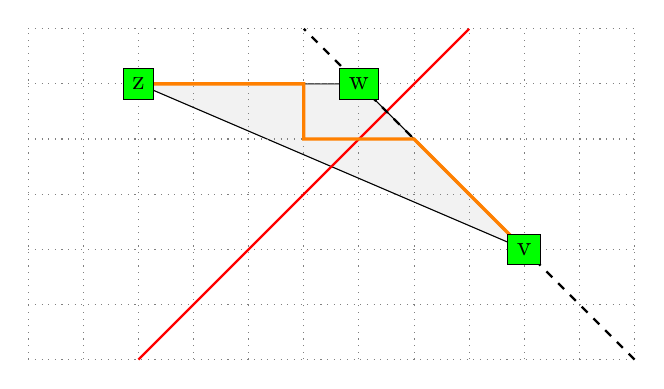
\begin{tikzpicture}[scale=0.7]
    %\draw[fill=red!10] (0,6) -- (0,0) -- (2,4) -- cycle;
    %\draw[fill=blue!10] (2,1) -- (2,4) -- (3,5) -- (6,5) -- (9,2) -- (8,1) -- cycle;
    %\draw[fill=yellow!10] (3,6) -- (3,5) -- (6,1) -- (6,2) 
      -- cycle;
    %\draw[fill=green!10] (7,6) -- (12,6) -- (10,4) -- (5,4) 
      -- cycle;
    \draw[fill=gray!10] (2,5) -- (6,5) -- (9,2) -- cycle;
    \draw[color=gray, style=dotted] (0,0) 
      grid[xstep=1cm, ystep=1cm] (11cm,6cm);
    \draw[red,thick] (2,0) -- (8,6); 
    \draw[dashed,thick] (11,0) -- (5,6);
    \draw[orange,very thick] (2,5) -- (5,5) -- (5,4) -- (7,4) -- (9,2); 
    %\draw[orange,thick] (2,5) -- (9,2); 
  	%\node at (2,1) [draw,fill=green] {};
  	\node at (6,5) [draw,fill=green] {w};
  	\node at (2,5) [draw,fill=green] {z};
  	\node at (9,2) [draw,fill=green] {v};
  	%\node at (7,4) [draw,fill=green] {\ };
  	%\node at (5,4) [draw,fill=green] {};
  \end{tikzpicture}
  \caption{The hypothetical line $l$ is marked in red. The chain line connecting $z$ and $v$ is marked in orange.}% and points} % $v,w$ are marked in blue and black, point $z$ is marked in yellow. }
  \label{gaphull}
  \end{center}
  \end{figure}